
%%% Uncomment for slide version
\documentclass[xcolor=dvipsnames]{beamer}
\setbeameroption{hide notes} % Only slides

%%% Uncomment for handout version
%\documentclass[handout]{beamer}
%\setbeameroption{show notes on second screen=right} % Both

\usepackage{enumitem}
\usepackage{listings}
\usepackage{adjustbox} % To incorporate code into Latex
\usepackage{multirow} % To merge multiple rows  in a table
\usepackage{soul} % To put in strikethrough text
\usepackage{array}
\usepackage{makecell}

\setbeamertemplate{note page}{\pagecolor{white}\insertnote}
\setbeamertemplate{footline}{}
\usetheme[progressbar=frametitle]{moloch}% modern fork of the metropolis theme
\setbeamercolor{background canvas}{bg=white}
\setbeamercolor{frametitle}{fg=black,bg=ProcessBlue!20}

\setbeamercolor{progress bar}{use=palette primary,fg=black,bg=black}
\setbeamercolor{note page}{bg=white} 
\setbeamertemplate{date}{}


\DeclareUnicodeCharacter{0313}{*************************************}

\setbeamertemplate{page number in head/foot}{}


\addtobeamertemplate{navigation symbols}{}{%
	\usebeamerfont{footline}%
	\usebeamercolor[fg]{footline}%
	\hspace{1em}%
	\insertframenumber/\inserttotalframenumber
}
\setbeamercolor{itemize item}{fg=black}
\setbeamercolor{itemize subitem}{fg=black}
\setbeamercolor{itemize subsubitem}{fg=black}

\newcommand\blfootnote[1]{%
	\begingroup
	\renewcommand\thefootnote{}\footnote{#1}%
	\addtocounter{footnote}{-1}%
	\endgroup
}

%%%%%%%%%%%%%%%%%%
%%%%%%%%%%%%%%%%%%
%%%%%%%%%%%%%%%%%%
%%%%%%%%%%%%%%%%%%
%%%%%%%%%%%%%%%%%%
%%%%%%%%%%%%%%%%%%
%%%%%%%%%%%%%%%%%%




\title{\Huge FRST302: Forest Genetics}
\author{\Large Lecture 4.1 -  Accelerating Tree Improvement I}
\date{\today}

\begin{document}
	\maketitle

\begin{frame}
\Huge Welcome to Module 4!
\end{frame}


\begin{frame}
\frametitle{Housekeeping}
\begin{itemize}
	\item[-] Module test will be a mix of multiple choice and short answer questions
	\item[-] The test questions will test your understanding of concepts and ask you to apply it
	\item[-] \textbf{Terminology} will be covered on lecture slides
	\item[-] \textbf{Concepts} will be covered in lectures 
	\item[-] If you are lost with the concepts or terminology make use of office hours, the Canvas Discussion board and ask questions in class!
\end{itemize}
\end{frame}




	\begin{frame}
		\frametitle{Recap}
			
		\begin{itemize}
			\item{\textbf{Module 1}} Genes, Genomes and Sequencing
			\item{\textbf{Module 2}} Population Genetics and Local Adaptation
			\item{\textbf{Module 3}} Quantitative Genetics and 20th Century Breeding \pause
			\vspace{20pt}
					\item{\textbf{Module 4}} Advancing Forest Genetics with Recent Technology
				\end{itemize}
	\end{frame}

\begin{frame}

%%%
\begin{columns}
	\begin{column}{0.6\textwidth}
		\centering 	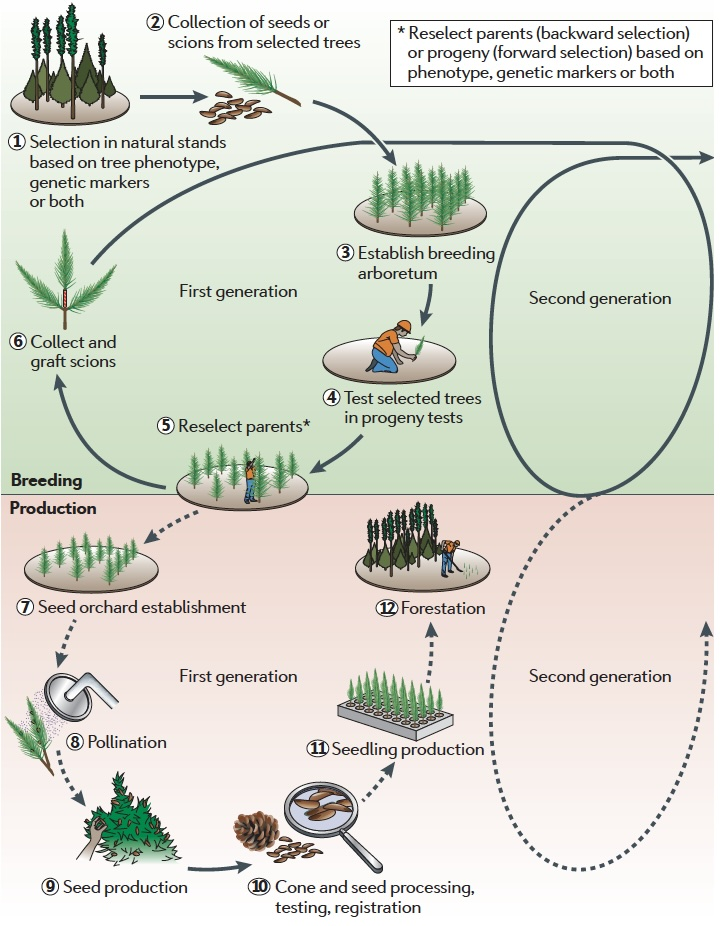
\includegraphics[keepaspectratio, width  = \textwidth]{img/treeImprovement}
	\end{column}
	\begin{column}{0.4\textwidth}
		\textbf{Conventional Tree Breeding\\}
		\pause
		Each cycle takes from 20-30 years!
	\end{column}
\end{columns}
\blfootnote{Image from Neale and Kremer 2011}
\end{frame}

\begin{frame}
\frametitle{Can We Afford to Take That Long?}
\centering
	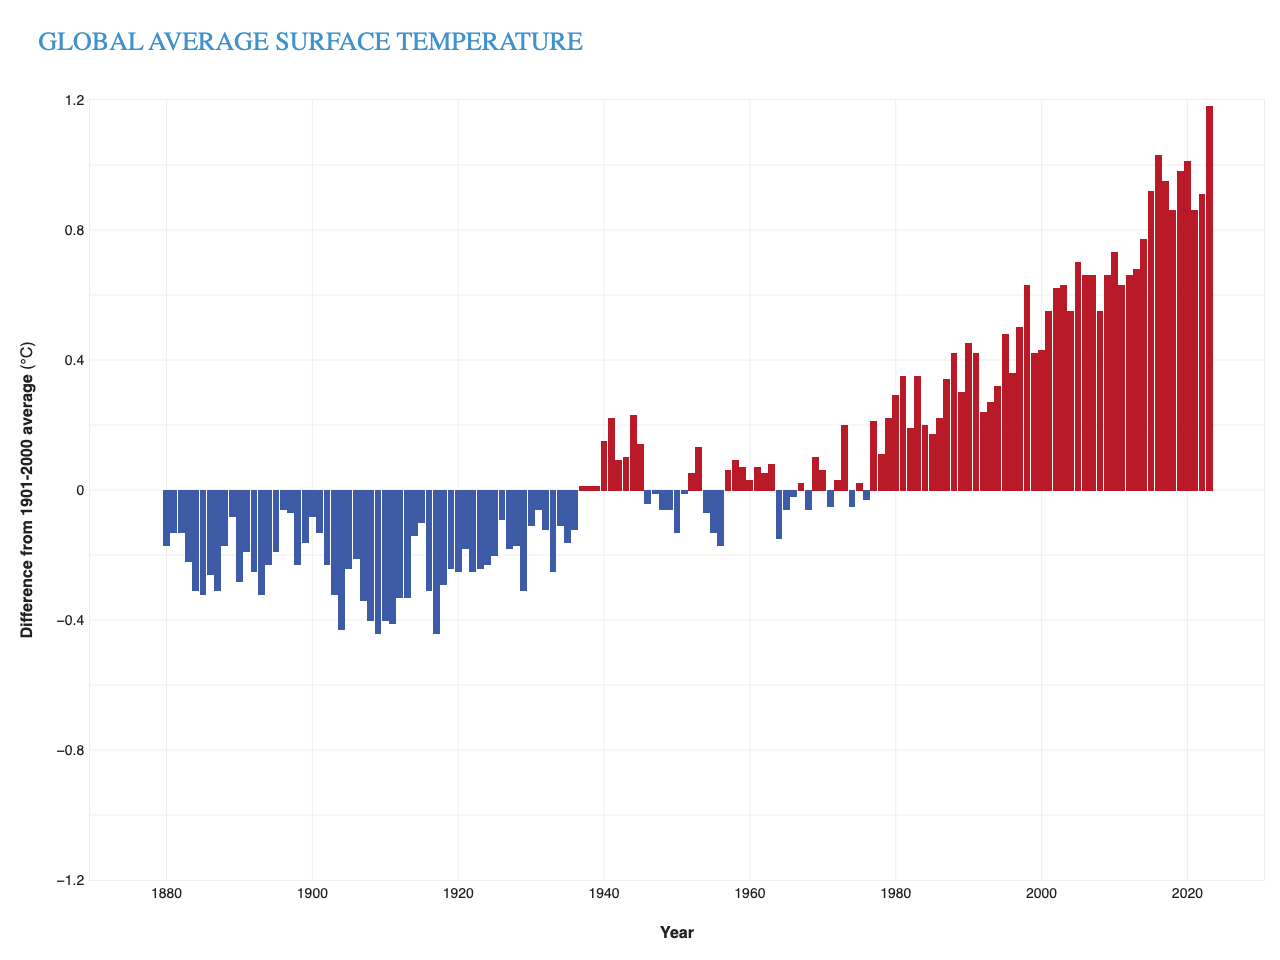
\includegraphics[keepaspectratio, width  = 0.8\textwidth]{img/graph_globalavgsurfacetemp}
	\blfootnote{\url{https://www.climate.gov/news-features/understanding-climate/climate-change-global-temperature} - \textit{Hopefully the webpage still exists...}}
\end{frame}




\begin{frame}
	\Huge How could you advance tree breeding with what you learned in the last three modules?
\end{frame}


\end{document}


%%%
	\begin{columns}
	\begin{column}{0.5\textwidth}
	\end{column}
	\begin{column}{0.5\textwidth}
	\end{column}
\end{columns}



